\documentclass[10pt]{article}
\usepackage[utf8]{inputenc}
\usepackage{kotex}
\usepackage{graphicx}
\usepackage{subfigure}
\usepackage{titling}
\setlength{\droptitle}{-2cm}
\usepackage{array}
\usepackage{amssymb}
\usepackage{amsmath}
\usepackage{siunitx} 
\usepackage{enumerate} 
\usepackage{pgfplots}
\usepackage{pgfplotstable}
\usepackage{tikz,pgfplots}
\usepackage{wasysym}
\usepackage{geometry}
\usepackage{authblk}
\usepackage{kotex}
\usepackage{bibunits}
\usepackage{tabularx}
\usepackage{hyperref}

\geometry{
    a4paper,
    total={170mm,257mm},
    left=20mm,
    top=20mm,
}

\title{\textbf{Artificial Intelligence: HW 2}}
\author{Jeong Min Lee}

\begin{document}
\maketitle

\section{Face Detection}
In this section, I will discuss the \textbf{face\_recognition()} method.

First, let's take a look at the result of \textbf{face\_recognition()}:
\begin{figure}[!h]
    \begin{center}
        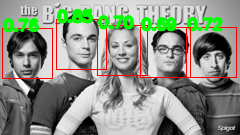
\includegraphics[scale=1.5]{./figures/result_face_detection.png}
    \end{center}
    \caption{Result of \textbf{face\_recognition()} applied to the given target and template.}
\end{figure}

As you can see, \textbf{face\_recognition()} produces highly accurate face detection results. 

Now, let me provide a brief explanation of how \textbf{face\_recognition()} works. The process consists of two main steps: collecting bounding boxes and applying non-maximum suppression. 

We begin by extracting HOG features from patches obtained from both the template and the target. These features are used to calculate the correlation or dot product after subtracting their averages. We save the coordinates of the top-left corner of bounding boxes along with their respective scores, provided their scores exceed 0.65.

Subsequently, we reduce the number of bounding boxes through non-maximum suppression. This is achieved by using the Intersection over Union (IoU) metric to determine whether bounding boxes are neighbors. The algorithm for non-maximum suppression is adapted from the article specified in the instructions. Calculating the IoU was also informed by a different article which proposed the specification. I had to adjust the IoU calculation code to accommodate the requirement that both input boxes have the same size. After applying non-maximum suppression, we obtain the final bounding boxes by removing the first element added for implementation purposes.

I would like to mention that I implemented \textbf{face\_recognition()} by modularizing the \textbf{non\_maximum\_suppression()} and \textbf{getIOU()} functions. However, the TAs requested that I implement \textbf{face\_recognition()} without introducing new functions. As a result, I embedded the code of these functions directly into \textbf{face\_recognition()}. This may lead to the redundancy of variables, and some might find the implementation less streamlined.


\end{document}
